\documentclass{article}[18pt]
\usepackage{../../../../format}
\lhead{Networks and Systems - Distributed Systems}


\begin{document}
\begin{center}
\underline{\huge Middleware Technologies and RMI}
\end{center}
\section{Middleware Technologies}
User perspective:
\begin{itemize}
	\item Hide users from the implementation details and the "distributed" nature
\end{itemize}
Developer perspective:
\begin{itemize}
	\item Hide DS developers from low-level details
	\item Provide common programming abstraction and infrastructure for constructing distributed applications
\end{itemize}
\section{Examples of middleware}
Service broker:
\begin{itemize}
	\item Serve as the prime interface for accessing a distributed system
	\item Identify or discover suitable remote component to serve the purpose
	\item Provide a variety of distributed system features, such as concurrency control, load distribution and fault tolerance
\end{itemize}
\section{Developing a distributed system with middleware}
Aims:
\begin{itemize}
	\item Focus on application logics
	\item Avoid implementing socket communication and dealing with network architecture and its dynamic changes
\end{itemize}
Middleware options:
\begin{itemize}
	\item Remote Procedure Call (RPC) - Inter-process communication; execute a remote function without the programmer coding the network communication
	\item Object-Oriented Middleware (OOM) - Extend the idea of RPC to allow remote invocation of objects
	\item Message-Oriented Middleware (MOM)
	\item Web Services
\end{itemize}
\subsection{Remote Procedure Call (RPC)}
\begin{itemize}
	\item Adapt traditional program paradigm, dividing a system into functions
	\item Mask remote function calls as being local, supporting distributed development
\end{itemize}
\begin{center}
	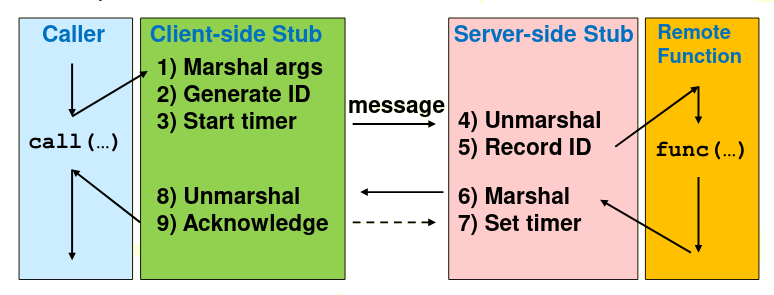
\includegraphics[scale=0.7]{RPC}
\end{center}
\begin{itemize}
	\item Request/reply paradigm usually implemented with message passing in RPC service
	\item Marshalling of function parameters and return value
\end{itemize}
\subsubsection{RPC Program development}
\begin{itemize}
	\item Server - Defines the service interface using an interface definition language (IDL), which specifies names, parameters, and types for all client-callable procedures
	\item Stub compiler - Reads the IDL declarations and produces two stub functions for each server function (server-side and client-side)
	\item Linking - Server programmer implements the service's functions and links with the server-side stubs. Client programmer implements the client program and links it with client-side stubs
	\item Operation  - Stubs manage all of the details of remote communication between client ans server
\end{itemize}
\subsubsection{Properties and Limitations}
Synchronous request/reply interaction:
\begin{itemize}
	\item Holds a connection open and waits until the response is delivered or the timeout period expires
	\item Tight coupling between client and server
	\item Client may block for a long time if server loaded
	\item Slow/failed clients may delay servers
\end{itemize}
Program paradigm: not object-oriented - invoke functions on servers - no encapsulation or inheritance support
\subsection{Object-Oriented Middleware (OOM)}
\begin{center}
	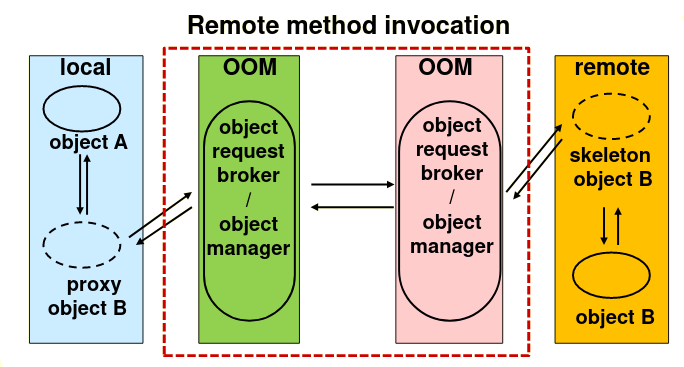
\includegraphics[scale=0.7]{OOM}
\end{center}
\begin{itemize}
	\item Objects can be local or remote
	\item Remote objects are visible through remote interfaces
	\item RMI masks remote objects as being local using proxy objects
	\item Object request broker identifies/discovers remote objects
\end{itemize}
\section{Java RMI}
\begin{itemize}
	\item Remote Method Invocation (RMI) is Java's implementation of object-to-object communication among Java objects to realise a distributed system
	\item RMI allows us to distribute our objects on various machines, and invoke methods on the objects located on remote sites
	\item \textbf{Advantage}: Dynamically invocate new versions of remote objects
	\item \textbf{Application}: Utilize very fast remote processors or any specialised resources
\end{itemize}
\begin{center}
	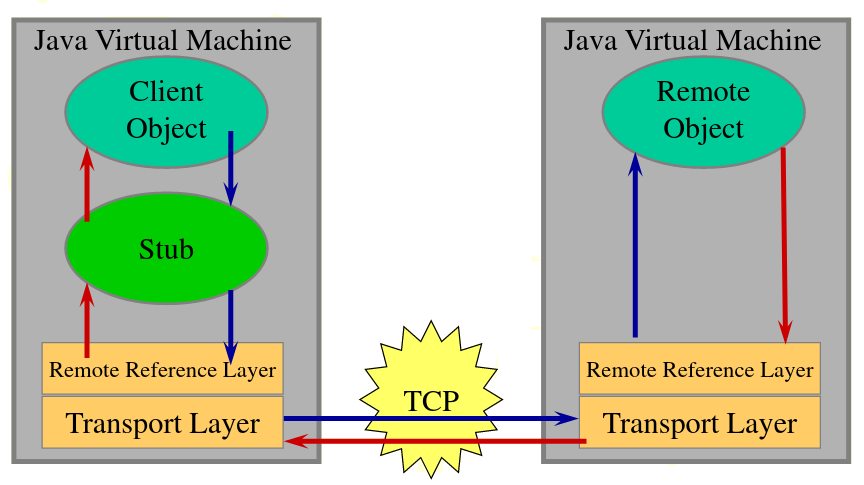
\includegraphics[scale=0.7]{RMI}
\end{center}
\subsection{RMI-based Application Development and Execution}
Development:
\begin{enumerate}
	\item Design the interface for the service
	\item Implement the methods specified in the interface
\end{enumerate}
Run time execution:
\begin{itemize}
	\item On the server
	\begin{itemize}
		\item Dynamically generate the stub
		\item Register the service by name and location
	\end{itemize}
	\item Client
	\begin{itemize}
		\item Look up the remote reference on the registry
		\item Use the service in an application
	\end{itemize}
\end{itemize}
\subsection{Registries (Object Broker)}

\end{document}